\section {System Setup and Development}
Para realizar os ensaios de convivência elaborou-se um arranjo de equipamentos, conforme ilustra a Figura
%To perform the coexistence tests, an arrangement of equipment was elaborated, as illustrated by figure
\ref{fig:SetupMedidas}. \par
%=========================================================
%=========================================================
O sistema foi operado através de um controlador embarcado responsável por rodar e gerenciar a aplicação desenvolvida. Para geração do \textit{Transport} \textit{Stream} (TS) utilizou-se um adaptador ASI (\textit{Asynchronous serial interface}) ligado a um modulador de TV digital (TVD) no padrão ISDB-T. Os sinais 5G foram transmitidos por um rádio definido por \textit{software} (RDS).\par

%The system was operated through an embedded controller responsible for rotating and managing the developed application. For generation of Texti{transport} Texti{stream} (TS) an ASI adapter (Texti{asynchronous serial Interface}) was used connected to a digital TV modulator (TVD) in the ISDB-T standard. 5G signals were transmitted by a radio set by texti{software} (RDS) .par

%==========================================================

O conjunto de sinais interferido e interferente foram agrupados, em meio confinado, utilizando um combinador de RF (Radiofrequência). Por fim o arranjo foi ligado aos receptores TVD. A observação da imagem foi realizada em uma televisão de uso doméstico. A conferência dos sinais no espectro eletromagnético e as medidas de potência de canal foram realizadas com um analisador digital de sinais. \par

%The set of interfered and interferent signals were grouped in a confined medium using an RF combiner (radiofrequency). Finally, the arrangement was connected to the TVD receptors. The observation of the image was performed on a home television. The Conference of Signals in the electromagnetic spectrum and the measurements of channel power were performed with a digital signal analyzer. par

%==========================================================

\begin{figure}[h!]
    \centering
    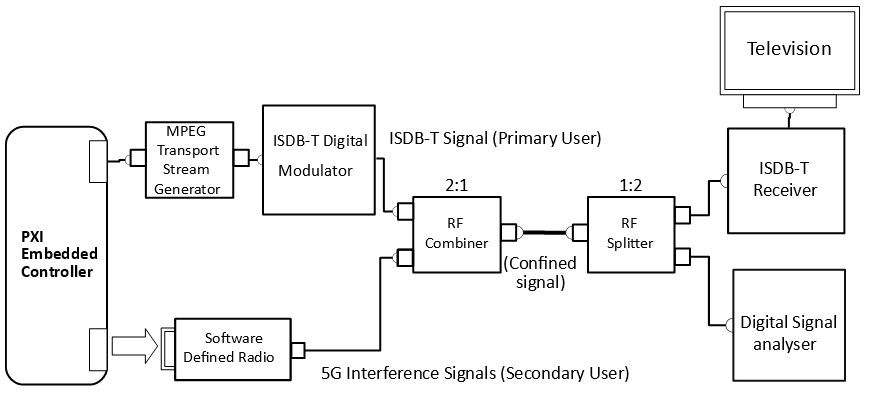
\includegraphics[width=0.45\textwidth]{Figures/setup_full_v3.jpg}
    \caption{Measurement setup proposed for coexistance procedures}
    \label{fig:SetupMedidas}
\end{figure}

%==========================================================

\subsection {Desenvolvimento da aplicação}
%==========================================================

A aplicação desenvolvida é composta por uma sessão de usuário e outra para interface com o rádio, como pode ser visto na Figura \ref{fig:DiagramaLabview}. O sistema gera um vetor de amostras em banda base\footnote{Referência de códigos para geração dos sinais 5G: \url{https://github.com/kit-cel/gr-gfdm}}, de acordo com seleção do usuário, modulado em uma das formas onda para a 5G descritas na secção \ref{sec:wave}. Uma vez que a configuração é feita, as amostras são então transferidas para o RDS. \par


%The application developed is composed of one user session and another for interface with the radio, as can be seen in Figure ref{fig: DiagramaLabview}. The system generates a vector of samples in band Basefootnote {code reference for generating 5G signals: url{https:/github.com/kit-cel/gr-gfdm}}, according to user selection, modulated in one of the waveforms for 5G described in section ref{sec: Wave }. Once the configuration is done, the samples are then transferred to the RDS. par


%==========================================================

\begin{figure}[h!]
    \centering
    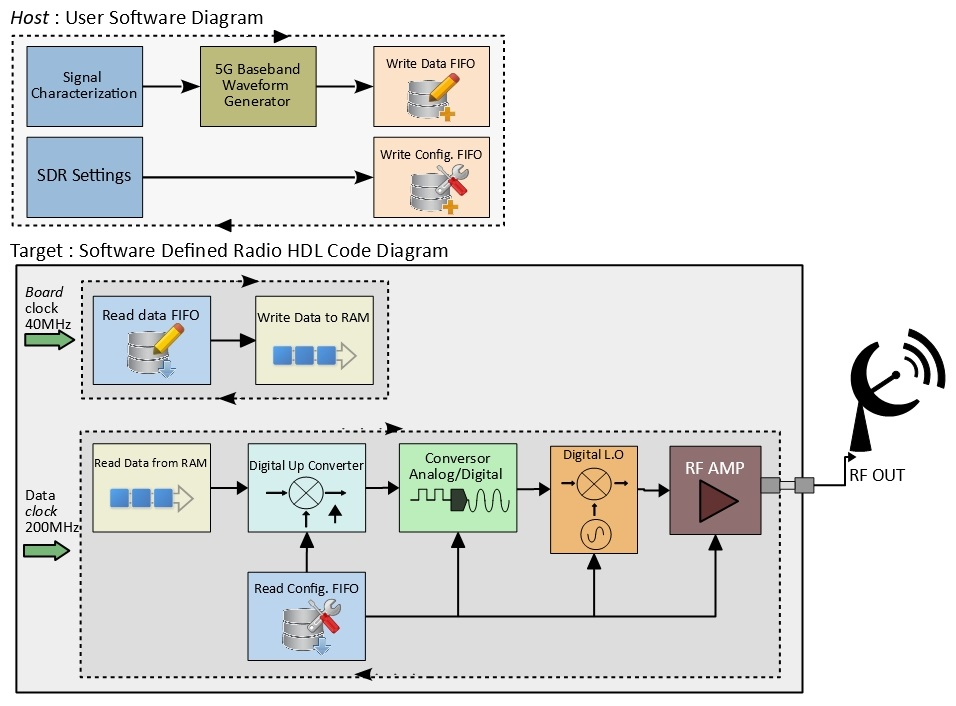
\includegraphics[width=0.45\textwidth]{Figures/Diagrama_Labview_full_v3.jpg}
    \caption{5G Waveform generator system block diagram}
    \label{fig:DiagramaLabview}
\end{figure}

%==========================================================

The data is written to a RAM and repeated sequentially until a new vector of samples is generated. The stream is converted to an intermediate frequency and then delivered to the analog digital converter. Finally the sequence is translated to channel frequency, and the RF transmission is performed. \par
%==========================================================


